\documentclass[12pt]{article}
\usepackage{tikz}
\usepackage{amsmath}
\usepackage{amssymb}
\usepackage{amsthm}
\usepackage{bm}
\usepackage{tcolorbox}
\tcbuselibrary{skins}
\usepackage{lipsum}
\usepackage[linesnumbered]{algorithm2e}
\makeatletter
\renewcommand{\@algocf@capt@plain}{above}
\makeatother
\usetikzlibrary{decorations.pathreplacing}
\usetikzlibrary{arrows}
\usetikzlibrary{snakes}
\usetikzlibrary{calc}
\let\emptyset\varnothing
\definecolor{hotpink}{rgb}{0.9,0,0.5}
\definecolor{deepgray}{gray}{0.35}
\definecolor{deepgray2}{gray}{0.25}
\definecolor{deepgray3}{gray}{0.10}
\definecolor{lightgray}{gray}{0.95}
\definecolor{lightgray2}{gray}{0.85}
\definecolor{purple1}{RGB}{239,229,244}
\definecolor{purple2}{RGB}{216,191,216}
\definecolor{lightblue}{rgb}{0.73,0.33,0.83}
\definecolor{lightpurple}{rgb}{.8,.2,.8}
\definecolor{textcolor}{rgb}{0,0,5}
\definecolor{blue1}{RGB}{187,217,238}
\definecolor{blue2}{RGB}{235,244,250}
\definecolor{yellow1}{RGB}{255,255,102}
\definecolor{blue3}{RGB}{63,40,96}
\definecolor{red1}{RGB}{255, 102, 102}
\definecolor{green1}{RGB}{102, 255, 102}
\newtheorem{lemma}{Lemma}
\newtheorem{theorem}{Theorem}
\newtheorem{definition}{Definition}
\theoremstyle{definition}
\def\proof{\par{\bf Proof}. \ignorespaces}
\def\qedsymbol{\vbox{\hrule\hbox{%
                     \vrule height1.3ex\hskip0.8ex\vrule}\hrule}}
\def\endproof{\qquad\qedsymbol\medskip\par}

% \usepackage{booktabs} % For formal tables
% \usepackage{cite}
\usepackage{url}
% \newtheorem{definition}{Definition}[section]
% \newtheorem{theorem}{Theorem}[section]
% \usepackage{algorithmic}
% \usepackage[cmex10]{amsmath}
\usepackage{amssymb}

\title{A Closer Look at Time-Preserving Paths on Evolving Graphs}

\author{Jiahao Chen and
Weijian Zhang
\thanks{%
  School of Mathematics,
The University of Manchester,
                Manchester, M13 9PL, England.
\texttt{weijian.zhang@manchester.ac.uk}.
}
}

\def\R{\mathbb{R}}
\def\C{\mathbb{C}}
\def\nbyn{n \times n}
\def\mbyn{m \times n}
\def\l{\lambda}
\def\norm#1{\|#1\|}
\def\normi#1{\|#1\|_1}
\def\normo#1{\|#1\|_{\infty}}
\def\Chat{\widehat{C}}
\def\e{eigenvalue}

% \DeclareMathOperator{\diag}{diag}   % Requires amsmath.
\def\diag{\mathop{\mathrm{diag}}}     % If not using amsmath.
\def\trace{\mathop{\mathrm{trace}}}   % If not using amsmath.

\def\At{\widetilde{A}}
\def\normt#1{\|#1\|_2}

% Note: this clashes with amsmath.
\def\bmatrix#1{\left[\matrix{#1}\right]}

\begin{document}

%\subtitlenote{The full version of the author's guide is available as
 % \texttt{acmart.pdf} document}


\maketitle

\begin{abstract}
This paper studies evolving graph centrality from the perspective of time-preserving paths. We describe time-preserving paths based on two dimensions of variation, namely static edges and causal edges.

A time-preserving path on evolving graphs makes implicit assumptions about the type of edges that a path traverses. For example, the path can count only static edges or can take account of both static edges and causal edges. In addition, the length of a time-preserving path can be either spatial or temporal.

We study the impact of different time-preserving paths on node centrality by varying the edge weights of static and causal edges.
We also compare evolving graph centrality with the aggregated static graph case to gain insight about the advantage of an evolving graph model.
We construct an evolving coauthor network from a collection of research papers for the experiments.
\end{abstract}

\section{Introduction}
\label{sec:introduction}

In the 1985 science-fiction film ``Back to the Future'', Marty McFly (played by Michael J. Fox) travelled back in time and accidentally changed history.
However, we cannot travel back in time or even send a message to the past.
An evolving graph in general is a time-dependent graph $G(t) = (V(t), E(t))$.
To traverse an evolving graph, one has to consider time. In particular, a path on an evolving graph needs to be time-preserving, meaning a node can not pass a massage (through an edge) to a node at a earlier time.

% time-respecting path
We represent an evolving graph as a time-ordered sequences of graphs, similar to the work of Tang and coworkers \cite{nicosia13, tang09, tang102, tang10} and Grindrod, Higham and coworkers \cite{grindrod13,grindrod11}. The idea is to divide the system's time span into temporal slices and regards it as a sequence of static graphs $G^{[t]}$, one for each layer. A node on a slice $G^{[t]}$ is represented by a pair $(v, t)$, where $v$ is a node of
$G^{[t]}$ and $t$ is the time stamp of the slice. A time-respecting path of length $n$ is a sequence of these node pairs $\langle (v_1, t_1), (v_2, t_2), \ldots ,(v_m, t_m)\rangle$, where $t_1 \le t_2 \le \cdots \le t_n$. Note if $t_i = t_j$, then $\langle (v_i, t_i), (v_j, t_j) \rangle$ is an edge at a temporal slice,  otherwise it is an edge linking nodes from different temporal slices.
We call edges of the first kind \emph{static edges} and of the second kind
\emph{causal edges}.
For example, in Figure \ref{fig:eg_shortest_path}
$\langle (1, t_1), (2, t_1) \rangle$ is a static edge at time stamp $t_1$ and $\langle (3, t_2), (3, t_3) \rangle$ is a causal edge between time stamp $t_2$ and time stamp $t_3$.
The difference between static edges and causal edges were first explicitly considered in \cite{chen16}.

\begin{figure}[h]
 \begin{center}
    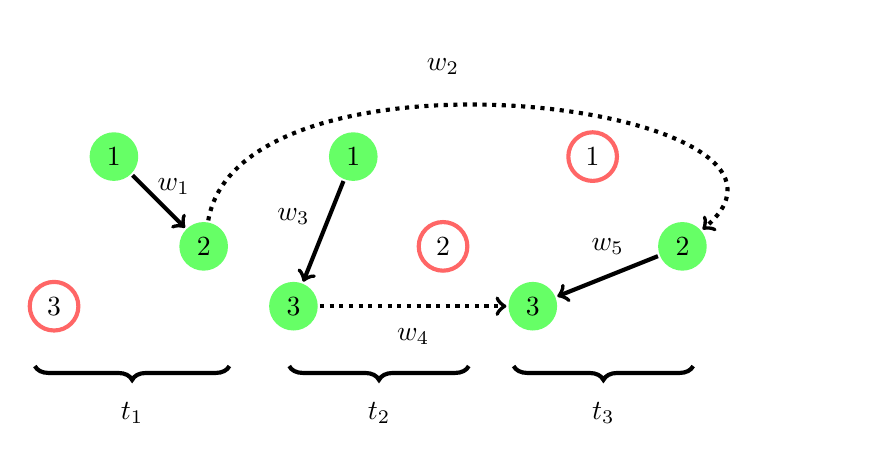
\begin{tikzpicture}[scale=.38, line width =1.5pt]
  \node[circle,fill=green1, minimum size=0.2cm] (n7) at (-5,7) {2};
  \node[circle,draw=red1, minimum size=0.2cm] (n8) at (-10,5) {3};
  \node[circle,fill=green1, minimum size=0.2cm] (n10) at (-8,10) {1};
  \node[circle,draw=red1, minimum size=0.2cm] (n6) at (3,7) {2};
  \node[circle,fill=green1, minimum size=0.2cm] (n4) at (-2,5) {3};
  \node[circle,fill=green1, minimum size=0.2cm] (n1) at (0,10) {1};
   \node[circle,fill=green1, minimum size=0.2cm] (n11) at (11,7) {2};
  \node[circle,fill=green1, minimum size=0.2cm] (n12) at (6,5)  {3};
  \node[circle,draw=red1, minimum size=0.2cm] (n14) at (8,10) {1};
  \node (w1) at (-6, 9) {$w_1$};
  \node (w2) at (3, 13) {$w_2$};
  \node (w3) at (-2, 8) {$w_3$};
  \node (w4) at (2, 4) {$w_4$};
  \node (w5) at (8.5, 7) {$w_5$};s
  \foreach \from/\to in {n10/n7, n1/n4, n11/n12}
   \draw[every edge,->] (\from) -- (\to);
 \draw[dotted,->](n4) -- (n12);
\draw[dotted,->](n7) to[out=80, in=40](n11);
\draw [decorate,decoration={brace,amplitude=5pt},xshift=-4pt,yshift=0pt]
(4,3) -- (-2,3) node [midway,yshift=-0.6cm]{ $t_2$};
\draw [decorate,decoration={brace,amplitude=5pt},xshift=-4pt,yshift=0pt]
(-4,3) -- (-10.5,3) node [midway,yshift=-0.6cm]{ $t_1$};
\draw [decorate,decoration={brace,amplitude=5pt},xshift=-4pt,yshift=0pt]
(11.5,3) -- (5.5,3) node [midway,yshift=-0.6cm]{ $t_3$};
    \end{tikzpicture}
\end{center}
\caption{An evolving directed graph with 3 time stamps $t_1$, $t_2$ and $t_3$.
At each time stamp, the evolving graph is represented as a graph.
The green filled circles represent active nodes while the red circles represent
inactive nodes. Directed edges in each time stamp are shown as black arrows and directed edges between graphs are shown as dotted arrows, where $w_1, w_2 \ldots w_5$ are edge weights.}
\label{fig:eg_shortest_path}
\end{figure}

It is natural to define the length of a path on a static graph as the number of nodes travelled through the path. For the weighted graph case, the length of a path is the total weight of all the edges in the path. We observe that static edges link nodes in space while causal edges link nodes in time. Hence we would like to distinguish temporal distance from spatial distance on an evolving graph: the length of a static edge is equal to the edge weight (or $1$ in the unweighted graph case); the length of a causal edge is the time distance between the two nodes. In the simplest case, the time-respecting path
$\langle (1, t_1) ,(2, t_1) , (2, t_3), (3, t_3)\rangle$ in Figure \ref{fig:eg_shortest_path} has length $4$ in total because two static edges $\langle (1, t_1) (2, t_1) \rangle$ and $\langle (2, t_3), (3, t_3) \rangle$ have length one, whereas $\langle (2, t_1) (2, t_3) \rangle$ traverse $2$ time stamps so has length $2$.

% We studies evolving graph centrality from the perspective of temporal network flows.
% Researchers have identified the time-preserving nature of such network flows, i.e.,
% we cannot travel between nodes from a later time to an early time.
% However, a closer look tells us there are subtle differences
% in previous papers

% How about a reverse time-preserving network flow?

% our contribution this paper
Borgatti noted in \cite{borgatti05} that the manner of traffic flow entails a new way to think about centrality. In particularly, the importance of a node in a network can not be determined without reference to how traffic flows through the network.
To develop a centrality algorithm on evolving graphs, one has to consider the manner of temporal traffic flow.
A time-preserving path on evolving graphs can be described by static edges, causal edges, or both.
Grindrod et al.'s definition of dynamic walk \cite{grindrod11} only counts static edges.
Tang et al. \cite{tang10s} measure a temporal shortest path in time unit (or causal edges) only. If a node can be reached by another node in $k$ time stamps then the distance between the two nodes is $k$. Chen and Zhang \cite{chen16} considered both static edges and causal edges in their definition of temporal path.


The aims of this paper are as follows. First, to identify the type of time-preserving path in a list of common evolving graph centrality measures. Second, to vary static and causal edge weights and analyze the impact on selected measures of centrality.
Third, to solve a real world problem using evolving graph centrality: identify key authors in an evolving coauthor network.
We carry out the experiment using the Julia dynamic network analysis package
EvolvingGraphs.jl (\url{https://github.com/EtymoIO/EvolvingGraphs.jl}).
We use the research paper data gathered from Etymo (\url{https://etymo.io}), a visual search engine for data scientists.


% \section{Background}
% \label{sec:preliminaries}
%
% Let $G$ be a directed graph with $n$ nodes with the corresponding adjacency matrix
% $A \in \R$.
%
% A \textbf{walk} of length $r$ from node $i_1$ to node $i_{r+1}$ is a sequence of edges
% $(i_1, i_2), (i_2, i_3), \ldots (i_r, i_{r+1})$.
%
%
% \subsection{Graph Centrality}
% \label{sec:katz-centrality}
%
% % definition of various graph centrality algorithms
% We review the Katz centrality here.
% Let $A$ be the adjacency matrix of a graph $G=(V,E)$ and $\rho(A)$ be the spectral radius of $A$. If $\alpha < 1/ \rho(A)$, then the Katz centrality vector of $G$ is
% \[
% (I - \alpha A)^{-1}e.
% \]
%
% The \emph{betweenness centrality} of a node $i$ in a static graph is defined as
% $$
% C_i = \sum_{j \in V}\sum_{k \in V, k \ne j} \frac{\rho_{jk}(i)}{\rho_{jk}},
% $$
% where $\rho_{jk}$ is the number of shortest paths from node $j$ to node $k$, while $\rho_{jk}(i)$ is the number of shortest paths from node $j$ to node $k$ that pass through node $i$

% The \emph{communicability betweenness centraltiy} \cite{estrada09} for a node $i$ is defined as
% $$
% C_i = C_N\sum_p \sum_q \frac{\exp(A)_{p,q} - \exp(A - E(i))_{p,q}}{\exp(A)_{p,q}},
% $$
% where $C_N = \frac{1}{(N-1)^2 - (N-1)}$ is a normalizing factor and $E(i)$
% has nonzeros only in row and column $i$, and in such row and column has $-1$ wherever $A$ has $1$. Similarly, the \emph{resolvent betweenness centrality} for node $i$ is defined as
% $$
% C_i = C_N\sum_p \sum_q \frac{(I - \alpha A)^{-1}_{p,q} - (I - \alpha(A - E(i)))^{-1}_{p,q}}{(I - \alpha A)^{-1}_{p,q}}.
% $$
% \subsection{Eigenvector Centrality}
% \label{sec:eigenv-centr}


% Given an adjacency matrix $A$ of a graph $G$, eigenvector centrality is defined as the dominant eigenvector of $A$, i.e.,
% \[
% \lambda v = Av,
% \]
% where $\lambda$ is the dominate eigenvalue of $A$ and $v$ is the corresponding eigenvector. Variations of eigenvector centrality includes Katz centrality \cite{katz53}, PageRank \cite{page99}, Hubbell's clique identification \cite{hubbell65}, Friedkin's actors' network centrality \cite{friedkin91}.
% In general, all eigenvector-like centrality are influence measures, meaning that even if a node $a$ only influences one node $b$, who influences many other nodes, then $a$ is highly influential.

% Let $A$ be the adjacency matrix of a graph $G = (V,E)$, i.e., $A_{i,j} = 1$ if node $i$ is linked to node $j$ and $A_{i,j} = 0$ otherwise. The idea of eigenvector centrality is that
% each node's centrality is the sum of the centrality values of the nodes that it is connected to. In other words, the relative centrality of node $v$ can be defined as
% \[
% x_v = \frac{1}{\lambda}\sum_{t \in M(v)} x_t = \frac{1}{\lambda}\sum_{t \in G} A_{v, t}x_t,
% \]
% where $M(v)$ is the set of neighbor nodes of $v$. We can write it in matrix notation as
% \[
% \lambda x = Ax.
% \]
% The eigenvector centrality of $G$ is the dominant (or principle) eigenvector of $A$.
% One may ask why we choose dominant eigenvector not any other eigenvectors? The answer comes from Perron-Frobenius Theorem (more details later).

% In \cite{bonacich91}, Bonacich prove the following theorem.
% \begin{theorem}
%   Assume that a symmetric non-negative matrix $A$ has a single largest eigenvalue $\lambda_1$ and its corresponding eigenvector $v_1$. Let $e$ be a column vector of ones. The infinite sum $A + \beta A^2 + \beta^2 A^3 + \beta^3 A^4 + \cdots$ converges
% if $|\beta| < 1/ \lambda_1$. Moreover, as $\beta$ approaches $1/\lambda_1$ from below,
% $(1-\beta\alpha_1)(A+ \beta A^2 + \beta^2 A^3 + \beta^3 A^4 + \cdots)e$ approaches $v_1$.
% \end{theorem}
% In other words, the eigenvector centrality of $G$ can be thought as proportional to an
% infinite sum
% \begin{equation}
% \label{eq:s}
% Se = Ae+ \beta A^2e + \beta^2 A^3e + \beta^3 A^4e + \cdots.
% \end{equation}
% Note however if $\beta = 1/\lambda_1$, the series does not converge.
% Eq. \eqref{eq:s} offers great flexibility to think about related centrality measures.
% For example, in the PageRank case
% \[
% r = Gr,
% \]
% where $G$ is a stochastic matrix. Then
% \[
% Se = Ge + \beta G^2e + \beta^2 G^3e + \beta^3 G^4 e + \cdots
% \]
% converges to $r$ as $\beta$ approaches $1$ from below.

% Note when $\alpha < 1/\rho(A)$, the spectral radius of $A$,
% \[
% (I - \alpha A)^{-1} = I + \alpha A + \alpha^2 A^2 + \alpha^3 A^3 + \cdots.
% \]
% Hence from eq. \eqref{eq:s} we have
% \[
% \beta Se + 1 = (I - \beta A)^{-1}e.
% \]
% This means eigenvector centrality can interpreted as Katz centrality with special chosen parameter value $\beta$. We mention that Aprahamian et. al. \cite{ahh16} consider selecting the Katz parameter based on the objective of matching the centrality of the exponential counterpart.


% \textbf{WZ:} some analysis need to be done on the relationship between
% $\beta$ and $v_1$. Derive some upper or lower bounds.

% %katz case
% Suppose we let
% \[
% S = A + \alpha_1^{-1} A^2 + \alpha_1^{-2} A^3 + \cdots,
% \]
% then $u = Se$ is proportional to the eigenvector $v_1$.

% In PageRank's case
% \[
% r = Gr,
% \]
% which means $\alpha_1 = 1$.

% Since Katz centrality can be written as
% \[
% (1- \alpha A)
% \]
% so it can be regard as a special case of eigenvector centrality.

% % \subsection{The Datasets}
% % \label{sec:datasets}

% % The data is a list of papers with associated information, including author names, affiliation, journal, and year of publication, and the full text content. We will test our algorithms on a collection of articles from, NIPS, an
% d ICLR.

% \subsection{Author Name Disambiguation}
% \label{sec:auth-name-disamb}

% We follow the idea from \cite{martin13} to disambiguate author names.

% \section{Eigenvector Centrality on Evolving Graphs}
% \label{sec:centr-algor}

% Let $A^{[t]}$ be the corresponding graph $G^{[t]}$ at a time label $t$. In \cite{grindrod11},
% Grindrod et. al. observes that the matrix product $A^{[t_1]}A^{[t_2]}\cdots A^{[t_w]}$ has
% $(i,j)$ element that counts the number of dynamic walks of length $w$ from node $i$ to node $j$ on which the $m$-th step of the walk takes place at time $t_m$. Therefore, the Katz centrality for evolving graphs can be written as
% \[
% Q = (I - \alpha A^{[0]})^{-1}(I - \alpha A^{[1]})^{-1} \cdots (I - \alpha A^{[m]})^{-1}.
% \]

% Follow the discussion from Section \ref{sec:eigenv-centr}, we can generalize eigenvector centrality and PageRank on evolving graphs.

\section{Time-Preserving Paths}
\label{sec:time-pres-paths}

We now describe time-preserving paths in more detail. We follow the definition of
\emph{evolving graph}, \emph{temporal node} and \emph{active node} in \cite{chen16}.

\begin{definition}
  An \textbf{evolving graph} $G_n$ is a sequence of (static) graphs
$G_n = \langle G^{[1]}, G^{[2]},  \ldots ,G^{[n]} \rangle$ with associated time stamps
$t_1, t_2, \ldots, t_n$ respectively. Each $G^{[t]} = (V^{[t]}, E^{[t]})$ represents a (static) graph labeled by a time t.
\end{definition}

Note the node sets $V^{[t]}$ can change over time, i.e., nodes may appear or disappear at a particular time stamp.
For example, in Figure \ref{fig:eg_shortest_path}, at time stamp $t_1$, $V^{[1]} = \langle 1, 2 \rangle$ and $E^{[1]} = \langle (1,2) \rangle$. Each graph $G^{[t]}$ can be represented by its adjacency matrix $A^{[t]}$.
We can represent $G_n$ by a list of adjacency matrices $A_n = \langle A^{[1]}, A^{[2]}, \ldots, A^{[n]} \rangle$.


\begin{definition}
  A \textbf{temporal node} is a pair (v, t), where $v \in V^{[t]}$ is a node at a time $t$.
\end{definition}

%At each time stamp, we only count temporal nodes that connects by an edge.

\begin{definition}
  A temporal node $(v, t)$ is an \textbf{active node} if there exists at least one edge $e \in E^{[t]}$ that connects $v \in V^{[t]}$ to another node $w \in V^{[t]}, w\ne v$. Otherwise it is called an inactive node.
\end{definition}

In Figure \ref{fig:eg_shortest_path}, the filled green circles are active nodes. For the adjacency matrix representation, a node $i$ is active at time stamp $t$, then
the $i$th row or the $i$th column of $A^{[t]}$ has at least one none-zero entry.
 In general, a time-preserving path can be defined as follows.

\begin{definition}
A \textbf{time-preserving path}  of length $m$ on an evolving graph $G_n$ is a time-ordered sequence of active nodes, $\langle (v_1, t_1), (v_2, t_2), \ldots, (v_m, t_m) \rangle$, where $t_1 \le t_2 \le \cdots \le t_m$ and
$v_i = v_j$ if and only if $t_i \ne t_j$.
\end{definition}

Note $\langle (v_i, t_i), (v_j, t_i) \rangle$ represents a static edge on graph $G^{[t_i]}$ while $\langle (v_i, t_i), (v_i, t_j) \rangle$ represents a causal edge from time stamp $t_i$ to time stamp $t_j$.

\begin{definition}
A \textbf{static edge} $\langle (v_i, t), (v_j, t)\rangle$ is a pair of elements of $V^{[t]}$, i.e., $v_i \in V^{[t]}$ and
$v_j \in V^{[t]}$.
 A \textbf{causal edge} $\langle (v, t_i), (v, t_j)\rangle$ is a pair of the same node at different time stamps.
\end{definition}

We can denote a \emph{weighted static edge} as $\langle (v_i, t), (v_j, t), w_s \rangle$ and a \emph{weighted causal edge} as $\langle (v, t_i), (v, t_j), w_t \rangle$.
Here $w_s$ represents the spatial distance between the two nodes $v_i$ and $v_j$; $w_t$ represents the
temporal distance of $v$ at different time stamps.
In Figure \ref{fig:eg_shortest_path}, the black arrows represent static edges and the dotted arrows represent causal edges.
Suppose we assign all the static edge weight to be $1$ and
assign the causal edge to be the number of time stamps between the pair. Then in Figure \ref{fig:eg_shortest_path}
the edge weight between $(1, t_1)$ and $(2, t_1)$ is $1$ and the edge weight between $(2, t_1)$ and $(2, t_3)$
 is $2$.

A time-preserving path can traverse both causal edges and static edges.
We will see in the next section that evolving centrality measures make implicit assumptions about the type of edges in the
time-preserving path that is used.


\subsection{Reverse Temporal Flows}
\label{sec:reverse-temp-flows}

We can not travel back in time. But reversing the direction of temporal flows can help
identify the ``hub'' nodes or the source of the flows. The authority score of a page is
proportional to its importance, and the hub score describes the quality of a page as a link collection of important related pages \cite{kleinberg99}.
Indeed, reverse PageRank has
been studied by \cite{bar08, fogaras03, gleich15}. In reverse PageRank we compute PageRank on the graph with reversed direction, i.e., reverse the direction of each edge $(i,j)$ to $(j, i)$.
Fogaras \cite{fogaras03} shows that Reversed Page Rank scores express hub quality.


Recall a time-preserving path is a time-ordered sequence of active nodes. Here we define a \emph{reversed temporal path} to be a reversed time-ordered sequence of active nodes, i.e.,
$t_1 \ge t_2 \ge \cdots \ge t_m$.


\section{Relation to Centrality Measures}
\label{sec:topol-temp-flow}

In \cite{tang10s}, a temporal shortest path is measured in time units only, i.e., if node
$v_i$ can reach node $v_j$ in $k$ time steps then the distance between node
$v_i$ and $v_j$ is $k$. We can apply temporal breadth first
search (BFS) \cite{chen16} to discover the temporal paths and then only take account of the temporal difference between the first node $(v_1, t_1)$ and the last node $(v_n, t_n)$, i.e., $t_n - t_1$.

If we use this definition of temporal path for the temporal Katz centrality introduced in
\cite{grindrod11}, we have a new centrality measure.
In the matrix form, the nonzero entries of $A^{[t_i]} A^{[t_{i+1}]}$ counts all the temporal paths of length $1$, and
$A^{[t_i]}\cdots A^{[t_j]}$, where $i < j$ counts all the temporal paths of length $j -i$.
For example, $A^{[1]}A^{[4]}$, $A^{[1]}A^{[1]}A^{[4]}$ and $A^{[1]}A^{[2]}A^{[3]}A^{[4]}$ are all walks of length 3.
In the original Katz centrality, the `attenuation' factor $\alpha$ is imposed on the
number of walks, i.e., longer walks has smaller effect to the overall rating.
Hence the final result is the summation of all products of the form
\[
\alpha^k A^{[i]} \cdots A^{[i+k]}
\]
% Note this can not be written in \eqref{eq:katz}, as discussed in Section \ref{sec:temp-katz-centr}.


Another definition of temporal path was introduced by \cite{chen16}. Here
both static edges and causal edges are considered. We can represent an evolving graph by a block adjacency matrix, as shown in Section \ref{sec:centr-block-adjac}. Centrality on this block matrix gives the importance of each node at all time stamps. We can average these rating at different time stamps to
get the final rating.


We review a few well-known measures of evolving graph centrality.
(Design a simple example and discuss it in each case below.)
\subsection{Temporal Katz Centrality}
\label{sec:temp-katz-centr}

The Katz Centrality is a measure of importance

In \cite{grindrod11}, Grindrod et al. define a \emph{dynamic walk} of length $m$ from
node $v_1$ to node $v_{w+1}$  as a sequence of edges
$(v_1, v_2), (v_2, v_3), \ldots (v_w, v_{w+1})$ and a non-decreasing sequence of times
$t_{r_1} \leq t_{r_2} \leq \cdots \leq t_{r_w}$ such that the adjacency matrix at time stamp
$r_m$, i.e., $A_{i_m, i_{m+1}}^{[r_m]} \ne 0$. Note that in this definition the authors only take account of the static edges and the length of a dynamic walk is determined by the number of static edges.

The Katz centrality is based on a sequence of matrix products
\begin{equation}
\label{eq:katz}
Q = (I - \alpha A^{[0]})^{-1}(I - \alpha A^{[1]})^{-1} \cdots (I - \alpha A^{[M]})^{-1}.
\end{equation}
The $i$th row and column sums
$$
C_i^{broadcast} = \sum_{k=1}^n Q_{ik}, \quad C_i^{receive} = \sum_{k=1}^n Q_{ki}
$$
are the broadcast centrality and receive centrality of node $i$.

\subsection{Temporal Betweenness Centrality}
\label{sec:temp-betw-centr}

Recall that betweenness centrality of a node in a static graph is defined by counting the fraction of shortest paths that traverse it.
We could extend
betweenness centrality on evolving graphs by replacing shortest paths with temporal shortest paths \cite{nicosia13}.
\begin{equation}
  \label{eq:bet1}
C_i^{betweenness} = \sum_{j \in V}\sum_{k \in V, k \ne j}\frac{\alpha_{jk}(i)}{\alpha_{jk}},
\end{equation}
where $\alpha_{jk}$ represents the number of temporal shortest paths from node $j$ to node $k$ and $\alpha_{jk}(i)$ represents the number of temporal shortest paths from node $j$ to node $k$ that pass through the node $i$.

One may want to take into account the length of time a node passes a message. The temporal betweenness centrality of the node $i$ at time stamp $t_m$ is defined as
\begin{equation}
  \label{eq:bet2}
  C_i^{betweenness}(t_m) = \sum_{j\ne i}\sum_{k\ne j, k\ne i}\frac{U_{j,k,t_m}(i)}{\alpha_{j,k}},
\end{equation}
where, as before, $\alpha_{j,k}$ represents the number of temporal shortest paths from $j$ to $k$ and $U_{j,k,t_m}(i)$ represents the number of temporal shortest paths from $j$ to $k$ in which node $i$ is traversed from
the path in the time stamp $t_m$ or a previous time stamp $t_{m-1}$. Then
average temporal betweenness of node $i$ is then defined as
$$
  C_i^{betweenness} = \frac{1}{M}\sum_m C_i^{betweenness}(t_m).
$$
Note \eqref{eq:bet1} only takes account of static edges while \eqref{eq:bet2} takes account of both static edges and causal edges.


\subsection{Temporal Closeness Centrality}
\label{sec:temp-clos-centr}

Let $d_{ij}$ be the length of a temporal shortest path from $i$ and $j$ in an evolving graph. Then
the closeness centrality of a node $i$ is defined
$$
C_i^{closeness} = \frac{N-1}{\sum_j d_{ij}}.
$$
Note that this depends on how we define the length of temporal shortest path. The closeness centrality can takes account of only static edges, only causal edges, or both.


\subsection{Centrality on a Block Adjacency Matrix}
\label{sec:centr-block-adjac}

In \cite{chen16}, we derive a block adjacency matrix representation of an evolvign graph.
If $E'$ is the set of causal edges and $\hat E$ is the set of static edges then
an evolving graph can be represented as
$$
\bm M_n =
\begin{pmatrix}
A^{[t_1]} & M^{[t_1, t_2]} & \ldots & M^{[t_1, t_n]} \\
0         & A^{[t_2]} & \ldots & M^{[t_2, t_n]} \\
          & \ldots    &        &     \\
0         & 0         & \ldots & A^{[t_n]}
\end{pmatrix},
$$
where $M^{[t_i, t_j]}$ is the matrix whose rows are labeled by $V^{[t_i]}$ and columns are labeled by $V^{[t_j]}$, and whose entries are
$$
  M_{uv}^{[t_i, t_j]} =
  \begin{cases}
    1 & \mbox{if} (u, v) \in E' \\
    0 & \mbox{otherwise}.
  \end{cases}
$$
The adjacency matrix blocks $A^{[t]}$ encode the static edge set $\hat E$, whereas the off-diagonal blocks $M^{[t_i, t_j]}$ encode the causal edge set $E'$.

(Need to justify the benefit of this approach.)
We can apply static graph centrality algorithms to $M_n$ and then take the average of ratings at each each time stamp. For example, we can construct the Google matrix
$G_n$ from $M_n$ and the ranking of the nodes can be found by solving
$$
 r= G_n r.
$$

For Figue \ref{fig:eg_shortest_path}, we have

\begin{align*}
V & = \{(1,\!t_1), (2,\!t_1), (1,\!t_2), (3,\!t_2), (2,\!t_3), (3,\!t_3)\},\\
\tilde E &= \{((1,\!t_1), (2,\!t_1)), ((1,\!t_2), (3,\!t_2)), ((2,\!t_3), (3,\!t_3))\},\\
E'  &= \{((1,\!t_1), (1,\!t_2)), ((2,\!t_2), (2,\!t_3)), ((3,\!t_2), (3,\!t_3))\}.
\end{align*}

and corresponding block adjacency matrix is

\[
\bm M_3 = \begin{pmatrix}
0 & 1 & 1 & 0 & 0 & 0 \\
0 & 0 & 0 & 0 & 1 & 0 \\
0 & 0 & 0 & 1 & 0 & 0 \\
0 & 0 & 0 & 0 & 0 & 1 \\
0 & 0 & 0 & 0 & 0 & 1 \\
0 & 0 & 0 & 0 & 0 & 0
\end{pmatrix}
\]

The static graph representation of Figure \ref{fig:eg_shortest_path} is shown in Figure \ref{fig:static}.

\begin{figure}[h]
 \begin{center}
   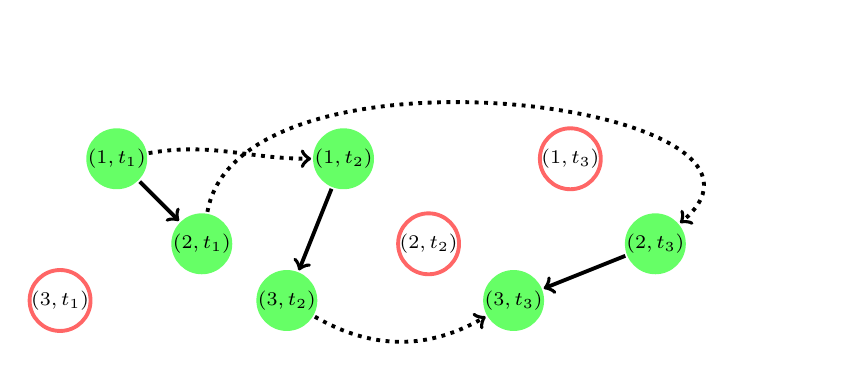
\begin{tikzpicture}[scale=.36, line width =1.4pt]
  \node[circle,fill=green1, minimum size=0.1cm, inner sep = 0pt] (n7) at (-5,7)
{\scriptsize $(2,t_1)$};
  \node[circle,draw=red1, minimum size=0.2cm, inner sep = 0pt] (n8) at (-10,5)
{\scriptsize $(3,t_1)$};
  \node[circle,fill=green1, minimum size=0.1cm, inner sep = 0pt] (n10) at (-8,10) {\scriptsize $(1,t_1)$};

  \node[circle,draw=red1, minimum size=0.2cm, inner sep = 0pt] (n6) at (3,7)
{\scriptsize $(2,t_2)$};
  \node[circle,fill=green1, minimum size=0.2cm,  inner sep = 0pt] (n4) at (-2,5)
{\scriptsize $(3,t_2)$};
  \node[circle,fill=green1, minimum size=0.2cm,  inner sep = 0pt] (n1) at (0,10)
{\scriptsize $(1,t_2)$};

   \node[circle,fill=green1, minimum size=0.2cm,  inner sep = 0pt] (n11) at (11,7)
{\scriptsize $(2,t_3)$};
  \node[circle,fill=green1, minimum size=0.2cm,  inner sep = 0pt] (n12) at (6,5)
{\scriptsize $(3,t_3)$};
  \node[circle,draw=red1, minimum size=0.2cm,  inner sep = 0pt] (n14) at (8,10)
{\scriptsize $(1,t_3)$};

  \foreach \from/\to in {n10/n7, n1/n4, n11/n12}
   \draw[every edge,->] (\from) -- (\to);
     \draw[dotted,->](n7) to[out=80, in=40] (n11);
  \draw[dotted,->](n10) to[out=10, in=180] (n1);
   \draw[dotted,->](n4) to[out=-30,in=-150] (n12);
    \end{tikzpicture}
\end{center}
\caption{A static graph corresponding to the evolving graph example of
Figure~\ref{fig:eg_shortest_path}. The green nodes are active nodes while the
red nodes are inactive nodes.
The black lines are edges in the static edge set $\tilde E$ and are encoded
algebraically in the diagonal blocks $A^{[t]}$ of the adjacency matrix $\bm M_3$.
The dotted lines are edges in the causal edge set $E'$ and are encoded algebraically in
the off-diagonal blocks $M^{[t_i, t_j]}$.
The graph containing all the edges and temporal nodes has adjacency matrix $\bm M_3$.}
\label{fig:static}
\end{figure}

\section{Experiments}
\label{sec:experiments}

In this section, we vary the edge
weights in both static and causal edges to study the impact of time-preserving paths on evolving graph centrality.
We also compare evolving graph centrality with the aggregated static graph case to gain insight about the advantage of evolving graph model.

\subsection{JMLR Coauthor Network}
\label{sec:jmlr-coauth-netw}


We construct the evolving coauthor network from Etymo (\url{https://etymo.io}).
We collected $1566$ publications published by Journal of Machine Learning Research (JMLR) from $2001$ to $2017$ with authors involved. We regard each year
as a time stamp and there are $17$ time stamps in total. At each time stamp, we
create a undirected edge (or two directed edges) between two authors if they have coauthored at least one paper.
(add results here.)

A second network is constructed by linking leading authors in different papers whose
ideas are similar. The resulting network represent the connectivity of ideas in all the research papers in the database.

(add results here.)


\subsection{Paper Subject Tag Network}

We tag our research articles by subjects. The subjects re provided by ACM Computing Classification System (also contains the superclass and subclass).

We can construct a time-dependent tag network by link tags in each articles. For example,
suppose a paper $p_1$ has three tags $t_1$, $t_2$, and $t_3$, where $t_1$ is a superclass of $t_2$ and $t_3$.
We link $t_2$ and $t_3$ in both direction and create a link from $t_1$ to $t_2$ and a link from $t_1$ to $t_3$.
The time stamp of these edges is the published date of the paper.


% subsection{Simulations}
% \label{sec:simulations-1}

% In \cite{borgatti05}, Borgatti simulate different types of walk flow on the network and
% compare the node statistics with the centrality measures.


% For katz centrality, eigenvector centrality, and PageRank (all on evolving graphs), we test all 3 different types of temporal flows.

% Problem setup: given a group of authors in an evolving graph, finding the most important authors. We use real dataset with real names.

% Build the evolving graph with author name disambiguation and apply the above algorithms.


% \subsection{Katz Centrality}
% \label{sec:katz-centrality-1}

% \subsection{Eigenvector Centrality}
% \label{sec:eigenv-centr-1}

% \subsection{PageRank}
% \label{sec:pagerank}



\section{Conclusion}
\label{sec:conclusion}

To write later.

\bibliographystyle{plain}
\bibliography{sigproc}

\end{document}

%%% Local Variables:
%%% mode: latex
%%% TeX-master: t
%%% End:
